\documentclass[../machine_learning_scikit.tex]{subfiles}

\begin{document}

    \chapter{Training Simple Machine Learning Algorithms for Classification}

    So, we will see basic algorithms for classification and some other useful things.

    \section{Introduction}

    In this section we will make use of the first two algorithmically described machine learning algorithms for classification: the \textbf{perceptron} and \textbf{adaptive linear neurons}.

    Frist, we'll start by implementing a perceptron step by step in Python and training it to classify different flower species in the iris dataset.

    \begin{obs}
        Using this algorithm and discussing the basics of optimization using adaptive lienar neurons layse the groundwork for using more sophisticated classifiers.
    \end{obs}

    The goals of this chapter are the following:
    \begin{itemize}
        \item Building an understanding of machine learning algorithms
        \item Using pandas, NumPy, and Matplotlib to read in, process, and visualize data
        \item Implementing linear classifiers for 2-class problems in Python
    \end{itemize}

    \section{Artificial Neurons: Early Stages of Machine Learning}

    Warren McCulloch and Walter Pitts published the first concept of a simplified brain cell, the so-called McCulloch-Pitts (MCP) neuron, in 1943 (A Logical Calculus of the Ideas Immanent in Nervous Activity by W. S. McCulloch and W. Pitts, Bulletin of Mathematical Biophysics, 5(4): 115-133, 1943).

    \begin{obs}[\textbf{Biological Neurons}]
        Biological Neurons are interconnected nerve cells in the brain that are involved in the processing and transmiting of chemical and electrical signals.
    \end{obs}

    \begin{figure}[h]
        \begin{minipage}{\textwidth}
            \centering
            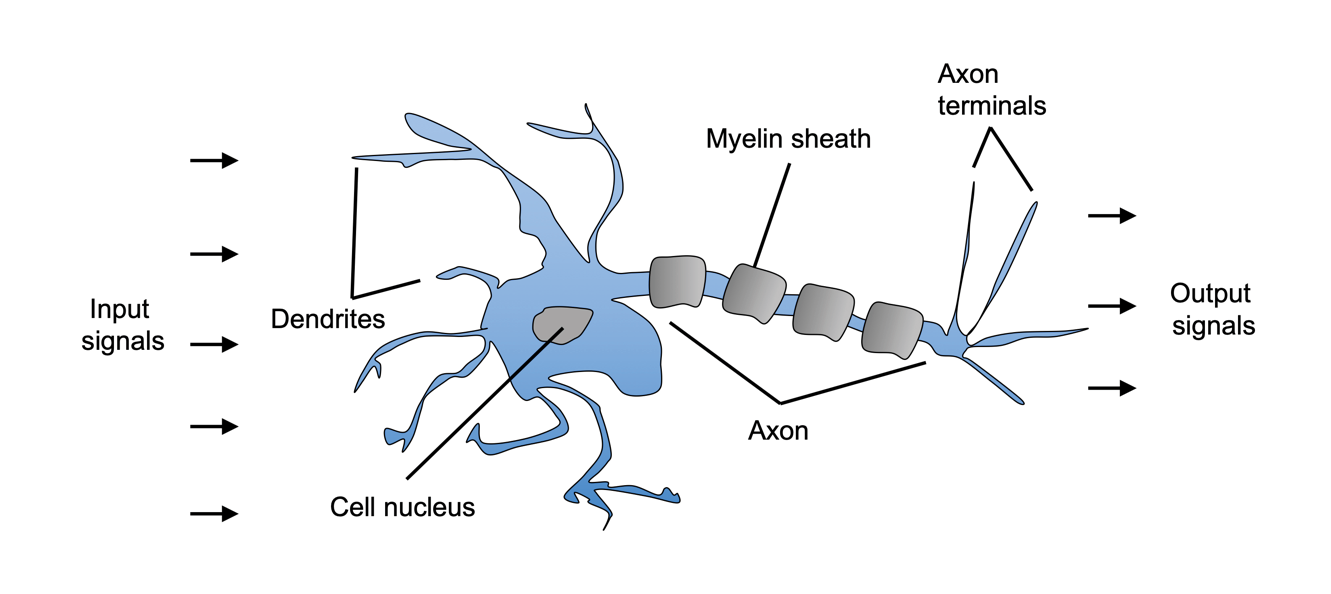
\includegraphics[scale=1]{images/nerve_cell.png} \\
            \caption{Biological Neuron.}
            \label{figure:biological_neuron}
        \end{minipage}
    \end{figure}

    \begin{idea}
        They described a nerve cell as a \textbf{simple logic gate with binary outputs}.
    \end{idea}

    Multiple signals arrive at the dendrites, they are then integrated into the cell body and, if the accumulated signals exceeds a certain threshold, an output signal is generated that will be passed on by the axon.

    \begin{obs}[\textbf{Perceptron Learning Rule}]
        Only a few years later, Frank Rosenblatt published the first concept of the \textbf{perceptron learning rule based} on the MCP neuron model (\textit{The Perceptron: A Perceiving and Recognizing Automaton} by F. Rosenblatt, Cornell Aeronautical Laboratory, 1957). With his perceptron rule, Rosenblatt \textit{proposed an algorithm that would automatically learn the optimal weight coefficients that would then be multiplied with the input features in order to make the decision of whether a neuron fires (transmits a signal) or not}.
    \end{obs}

    In the context of supervised learning and classification, \textit{such an algorithm could then be used to predict whether a new data point belongs to one class or the other}.

    \section{Formal Definition of an Artificial Neuron}

    We can put the idea of \textbf{articial neurons} into the context of a binary classification task with two classes: 0 and 1.

    \begin{mydef}[\textbf{Decision Function}]
        A \textbf{decision function} is a function $\cf{\sigma}{X}{\left\{0,1\right\}}$ that takes a linear combination of a certain input values (called $x$) and a corresponding weight vector (called $w$) , where $z$ is the net input:
        \begin{equation*}
            z=w_1x_1+w_2x_2+\dots+w_mx_m=\sum_{ i=1}^m w_ix_i
        \end{equation*}
        so, $\sigma(z)\in\left\{0,1\right\}$.
    \end{mydef}

    If the net input of a particular example is greater than a defined threshold (lets say $\vartheta\in\bbm{R}$, so $z\geq\vartheta$), we predict class 1, and class 0 otherwise. In the perceptron algorithm, the decision function, $\sigma(z)$ is a variant of a \textbf{unit step function}:
    \begin{equation*}
        \sigma(z)=\left\{
            \begin{array}{lr}
                1 & \textup{ if }z\geq\vartheta\\
                0 & \textup{ otherwise} \\
            \end{array}
        \right.
    \end{equation*}

    \begin{obs}
        We can modify the setup with a couple of steps. So, we make the \textbf{bias unit} $b=-\vartheta$, and we make:
        \begin{equation*}
            z'=w_1x_1+w_2x_2+\dots+w_mx_m+b=\vec{w}^T\vec{x}+b
        \end{equation*}
        And now replacing every input $z$ by $z'$ we obtain that:
        \begin{equation*}
            \sigma(z')=\left\{
                \begin{array}{lr}
                    1 & \textup{ if }z\geq0\\
                    0 & \textup{ otherwise} \\
                \end{array}
            \right.
        \end{equation*}
    \end{obs}

    \begin{obs}
        The transpose $A^T$ of matrix $A\in\mathcal{M}_{m\times n}$ is defined as:
        \begin{equation*}
            A^T=\left[
                \begin{array}{c c c c}
                    a_1^{(1)} & a_2^{(1)} & \cdots & a_n^{(1)} \\
                    a_1^{(2)} & a_2^{(2)} & \cdots & a_n^{(2)} \\
                    \vdots & \vdots & \ddots & \vdots \\
                    a_1^{(m)} & a_2^{(m)} & \cdots & a_n^{(m)} \\
                \end{array}
            \right]
        \end{equation*}
        where:
        \begin{equation*}
            A=\left[
                \begin{array}{c c c c}
                    a_1^{(1)} & a_2^{(1)} & \cdots & a_m^{(1)} \\
                    a_1^{(2)} & a_2^{(2)} & \cdots & a_m^{(2)} \\
                    \vdots & \vdots & \ddots & \vdots \\
                    a_1^{(n)} & a_2^{(n)} & \cdots & a_m^{(n)} \\
                \end{array}
            \right]
        \end{equation*}
    \end{obs}

    \begin{obs}[\textbf{Notation Problem}]
        This notation is horrible and differs from the one Mathmaticians use in all his textbooks, please, don't use this notation.
    \end{obs}

    \section{Perceptron Learning Rule}

    The whole idea behind the MCP neuron and Rosenblatt's thresholded perceptron model is to \textit{use a reductionist approach to mimic how a single neuron in the brain works}: \textbf{it either fires or it doesn't}. Thus, Rosenblatt's classic perceptron rule is fairly simple, and the perceptron algorithm can be summarized by the following steps:
    \begin{enumerate}
        \item Initialize the weights and bias unit to $0$ or small random numbers
        \item For each training example, $x^{(i)}$.
        \item Compute the output value, $\hat{y}^{(i)}$.
        \item Update the weight and bias unit.
    \end{enumerate}

    \begin{obs}[\textbf{Output Value}]
        Here, the \textbf{output value} is the \textbf{class label} \textit{predicted by the unit step function defined earlier}.
    \end{obs}

    The simultaneous update of each weight $w_j$ in the weight vector $\vec{w}$ can be formally written as:
    \begin{equation*}
        w_j\equiv w_j+\Delta w_j
    \end{equation*}
    and,
    \begin{equation*}
        b\equiv b+\Delta b
    \end{equation*}
    
    \begin{obs}[\textbf{Use of the Symbol $\equiv$}]
        Here, the symbol $\equiv$ states that the vlaue of the variable to the left is updated to that of the variable on the right.
    \end{obs}

    Where, the updated values (or \textbf{deltas}) are computed as follows:
    \begin{equation*}
        \Delta w_j=\eta(y^{(i)}-\hat{y}^{(i)})x_j^{(i)}
    \end{equation*}
    and,
    \begin{equation*}
        \Delta b=\eta(y^{(i)}-\hat{y}^{(i)})
    \end{equation*}

    \begin{obs}[\textbf{Notation Abuse}]
        This thing is absoultely ridicolus in terms of notation, the correct notation should be something like $\Delta w_j^{(i)}$, but since this variable is not going to be used anymore, we simply forgot about it, this is because in the process this variable is going to be updated every single time and we dont care about the different values depending on the $i$.
    \end{obs}

    Here, $\eta$ is a learning rate (usually between $0$ and $1$). $y^{(i)}$ is the \textbf{true class label} and $\hat{y}^{(i)}$ is the \textbf{predicted class label}.

    \begin{obs}
        The bias unit and all weights in the weight vector are updated simultaneously, which means that the predicted label $\hat{y}^{(i)}$ is not recomputed before the bias unit and all the wrights are updated via the respective update values, ,$\Delta w_j$ and $\Delta b$.
    \end{obs}

    \begin{exa}
        Concretely, for a two-dimensional dataset, we would write the update as:
        \begin{equation*}
            \begin{split}
                \Delta w_1&=\eta(y^{(i)}-\textup{output}^{(i)})x_1^{(i)}\\
                \Delta w_2&=\eta(y^{(i)}-\textup{output}^{(i)})x_2^{(i)}\\
                \Delta b&=\eta(y^{(i)}-\textup{output}^{(i)})\\
            \end{split}
        \end{equation*}
    \end{exa}

    \begin{enumerate}
        \item Before we implement the perceptron rule in Python, let's go through a simple thought experiment to illustrate how beautifully simple this learning rule really is. In the two scenarios where the perceptron predicts the class label correctly, the bias unit and weights remain unchanged, since the update values are 0:

        \item \textbf{When prediction is correct:}
        \begin{itemize}
            \item If $y^{(i)} = 0$ and $\hat{y}^{(i)} = 0$:
            \begin{align*}
            \Delta w_j &= \eta(0 - 0)x_j^{(i)} = 0 \\
            \Delta b &= \eta(0 - 0) = 0
            \end{align*}
            
            \item If $y^{(i)} = 1$ and $\hat{y}^{(i)} = 1$:
            \begin{align*}
            \Delta w_j &= \eta(1 - 1)x_j^{(i)} = 0 \\
            \Delta b &= \eta(1 - 1) = 0
            \end{align*}
        \end{itemize}

        \item \textbf{When prediction is wrong:}
        \begin{itemize}
            \item If $y^{(i)} = 0$ and $\hat{y}^{(i)} = 1$:
            \begin{align*}
            \Delta w_j &= \eta(0 - 1)x_j^{(i)} = -\eta x_j^{(i)} \\
            \Delta b &= \eta(0 - 1) = -\eta
            \end{align*}
            
            \item If $y^{(i)} = 1$ and $\hat{y}^{(i)} = 0$:
            \begin{align*}
            \Delta w_j &= \eta(1 - 0)x_j^{(i)} = \eta x_j^{(i)} \\
            \Delta b &= \eta(1 - 0) = \eta
            \end{align*}
        \end{itemize}

        \item To get a better understanding of the feature value as a multiplicative factor $x_j^{(i)}$, consider another example where $y^{(i)} = 1$, $\hat{y}^{(i)} = 0$, $\eta = 1$. Assume that $x_j^{(i)} = 1.5$ and this example is misclassified as class 0. In this case, we would increase the corresponding weight so that the net input $z = x_j^{(i)}w_j + b$ would be more positive the next time we encounter this example and thus more likely to be above the threshold of the unit step function to classify the example as class 1:
        \begin{align*}
        \Delta w_j &= (1 - 0) \times 1.5 = 1.5 \\
        \Delta b &= (1 - 0) = 1
        \end{align*}

        \item The weight update $\Delta w_j$ is proportional to the value of $x_j^{(i)}$. For instance, if we have another example $x_j^{(i)} = 2$ that is incorrectly classified as class 0, we will push the decision boundary by an even larger extent to classify this example correctly the next time:
        \begin{align*}
        \Delta w_j &= (1 - 0) \times 2 = 2 \\
        \Delta b &= (1 - 0) = 1
        \end{align*}

        \item The convergence of the perceptron is only guaranteed if the two classes are linearly separable, which means that the two classes can be perfectly separated by a linear decision boundary. If the two classes cannot be separated by a linear decision boundary, we can set a maximum number of passes over the training dataset (epochs) and/or a threshold for the number of tolerated misclassifications—the perceptron would never stop updating the weights otherwise.

        \item The perceptron receives the inputs of an example ($x$) and combines them with the bias unit ($b$) and weights ($w$) to compute the net input. The net input is then passed on to the threshold function, which generates a binary output of 0 or 1—the predicted class label of the example. During the learning phase, this output is used to calculate the error of the prediction and update the weights and bias unit.
    \end{enumerate}

    \section{Implementing a Perceptron Learning Algorithm in Python}

\end{document}